\documentclass[times,t]{beamer}
\usepackage{amssymb}
\usepackage{amsmath}
\usepackage{amsfonts}
\usepackage{lmodern} 
\input{sym.tex}
\setbeamertemplate{navigation symbols}{}

\title{ECE 417/598: Direct Linear Transform }
\author{Vikas Dhiman}
\date{March 23, 2022}
\DeclareMathOperator{\diag}{diag}
\begin{document}

\newcommand{\ubfu}{\underline{\bfu}}
\newcommand{\ubfx}{\underline{\bfx}}
\begin{frame}
  \titlepage
  \end{frame}


\begin{frame}{Implicit equation and parameteric representation of 3D plane} 

  \begin{minipage}{0.4\linewidth}
    Implicit equation of 3D plane
    \[ 
    \bfp^\top \ubfx = 0 \qquad \bfp \in \bbP^4, \ubfx \in \bbP^4 \]
    \end{minipage}
    \hfill
    \begin{minipage}{0.4\linewidth}
      % Let SVD of $\bfp^\top$ be \[ \bfp^\top = U \Sigma V^\top \],
      % and let
      % \[ V = \begin{bmatrix}
      %     \bfv_1 & \bfv_2 & \bfv_3 & \bfv_4
      %   \end{bmatrix}
      % \],
      % then the parameteric representation of the plane corresponding to the implicit equation is
      % \[
      %   \ubfx = \bfv_2 + \frac{\lambda_2}{\lambda_1} \bfv_3 + \frac{\lambda_3}{\lambda_1} \bfv_4
      %   \]
      %   or 
      Parameteric representation of 3D plane
        \[
          \ubfx = \bfv_2 + t_1 \bfv_3 + t_2 \bfv_4
        \]
        where $t_1, t_2 \in \bbR$ are the free parameters.
    \end{minipage}
\end{frame}

\begin{frame}{Implicit equation and parameteric representation of a 3D line} 
  \begin{minipage}{0.4\linewidth}
    Parameter representation of a 3D line
    \[ 
      \ubfx = \lambda \underline{\bfd} + \ubfx_0,
    \]
    where $\lambda \in \bbR$ is the free parameter, $\ubfx_0 \in \bbP^3$ is a point on
    the line and $\underline{\bfd} \in \bbP^3$ is the direction of the line.
  \end{minipage}
  \hfill
  \begin{minipage}{0.4\linewidth}
    Implicit equation of a 3D line
    \begin{align}
      \bfp_1^\top  \ubfx &= 0, & \bfp_2^\top \ubfx &= 0,
    \end{align}
    where $\bfp_1, \bfp_2, \ubfx \in \bbP^3$.
  \end{minipage}
\end{frame}

\begin{frame}
  \includegraphics[width=\linewidth]{media/lane-from-points.pdf}
  \begin{align*}
    \ubfx_1 &= [100, 98, 45,1]^\top\\
    \ubfx_2 &= [105, 95, 46, 1]^\top\\
    \ubfx_3 &= [107, 90, 47,1]^\top\\
    \ubfx_4 &= [110, 85, 43,1]^\top
  \end{align*}
  Find  the 3D line such that it is the ``closest line'' passing through
  $\bfx_1, \dots, \bfx_4 \in \bfP^3$.
\end{frame}

\begin{frame}{Parameteric representation through Range space}
  
\end{frame}


\begin{frame}{Homography}
  \includegraphics[width=\linewidth]{media/homography-maps-a-line-to-a-line.png}
\end{frame}

\begin{frame}{Examples  of  Homography}
  \includegraphics[width=\linewidth]{media/examples-of-homography.png}
\end{frame}

\begin{frame}
  \includegraphics[width=0.60\linewidth]{media/audi top view camera.jpg}
\end{frame}

\begin{frame}{Computing Homography}
  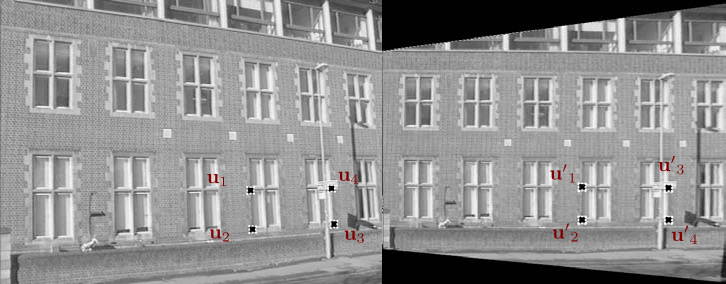
\includegraphics[width=\linewidth]{media/removing-perspective-distortion.png.pdf}
  \begin{align*}
    \ubfu_1 &= [100, 98, 1]^\top&
    \ubfu_2 &= [102, 95, 1]^\top\\
    \ubfu_3 &= [107, 90, 1]^\top&
    \ubfu_4 &= [110, 85, 1]^\top \\
    \ubfu'_1 &= [100, 98, 1]^\top&
    \ubfu'_2 &= [102, 95, 1]^\top\\
    \ubfu'_3 &= [107, 98, 1]^\top&
    \ubfu'_4 &= [110, 85, 1]^\top
  \end{align*}
  Find $H$ such that $\ubfu' = H\ubfu$ for any point on one image to another image.
\end{frame}

\begin{frame}{2D homography}
  Given a set of points $\ubfu_i \in \bbP^2$ and a corresponding set of
  points $\ubfu'_i \in \bbP^2$, compute the projective transformation that takes each
  $\ubfu_i$ to $\ubfu'_i$ . In a practical situation, the points $\ubfu_i$ and   $\ubfu'_i$  are points in two images
  (or the same image), each image being considered as a projective plane  $\bbP^2$.
\end{frame}

\begin{frame}{Solving for Homography }
\end{frame}


\begin{frame}{3D  to  2D camera projection matrix estimation}
  Given a set of points $\bfX_i$ in 3D space, and a set
  of corresponding points $\bfx_i$ in an image, find the 3D to 2D projective
  $\bfP$ mapping
  that maps $\bfX_i$ to $\bfx_i  =  \bfP\bfX_i$.
\end{frame}

\end{document}